\chapter{Lab 04 — California Housing Price Prediction}
\label{ch:lab04}

\section{Problem Definition}

\begin{problembox}
Predict \textbf{median house value} (USD) from census-block features using three regression models built \textit{from scratch} in pure NumPy. The dataset is the classic California Housing dataset (1990 census). Success criteria: \textbf{RMSE $< \$75{,}000$}, \textbf{R² $> 0.600$}, \textbf{MAPE $< 30\%$}. Every component — gradient descent, backpropagation, histogram-based tree splitting — is implemented from scratch without high-level ML libraries. The best-performing model (HistGradientBoosting) achieves RMSE $= \$51{,}648.807$, R² $= 0.795$, MAPE $= 21.383\%$.
\end{problembox}

\subsection{Dataset}
\begin{itemize}
  \item \textbf{Source:} California Housing (1990 census), 20,640 rows, 10 columns (9 numeric + 1 categorical).
  \item \textbf{Features:} 8 numeric (longitude, latitude, housing\_median\_age, total\_rooms, total\_bedrooms, population, households, median\_income) + 1 categorical (ocean\_proximity, 5 levels).
  \item \textbf{Target:} \texttt{median\_house\_value}, capped at \$500,001.
  \item \textbf{Split:} Stratified 80/20 on binned \texttt{median\_income} — 16,512 train, 4,128 test.
\end{itemize}

\section{Complete Workflow}

\subsection{Setup and Load Data}
Key libraries imported, project root resolved, \texttt{src/lab04} added to \texttt{sys.path} for custom module access. Raw CSV loaded: 20,640 rows, 10 columns. Descriptive commands (\texttt{.head()}, \texttt{.info()}, \texttt{.describe()}) provide the initial structural overview and reveal the variable scale disparities that necessitate standardization.

\subsection{Exploratory Data Analysis}

\subsubsection{Descriptive Statistics}
\texttt{df.describe()} confirms: \texttt{median\_house\_value} capped at \$500,001; \texttt{total\_rooms}, \texttt{total\_bedrooms}, and \texttt{population} are heavily right-skewed, with their 75th-percentile values far below their maxima — a hallmark of count distributions dominated by a few high-density census blocks. \texttt{ocean\_proximity} value counts reveal 5 categories with ISLAND containing only 5 samples, making it a candidate for merging with the nearest geographic neighbor.

\subsubsection{Missing Values}
Only \texttt{total\_bedrooms} has missing data: 207 rows out of 20,640 (1.003\%). This is well below the 10\% threshold where median imputation remains statistically valid and introduces negligible bias. \texttt{eda.plot\_missing\_values()} renders a bar chart confirming all other columns are complete.

\begin{figure}[H]\centering
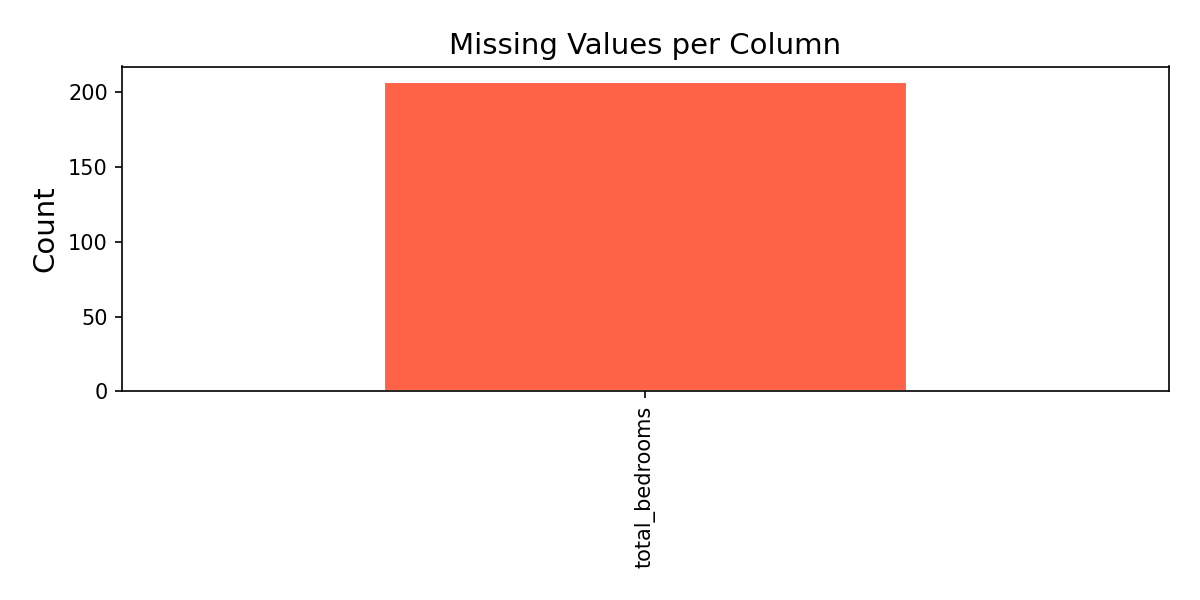
\includegraphics[width=0.72\textwidth]{figures/lab04/eda_01_missing_values.png}
\caption{Missing values bar chart — only \texttt{total\_bedrooms} shows gaps (207 rows, 1.003\%), all other columns are complete.}
\end{figure}

\subsubsection{Feature Distributions}
Histograms for all numeric features reveal characteristic patterns. Right-skewed count features (rooms, bedrooms, population, households) are candidates for $\log_{1p}$ transformation to reduce the leverage of high-count outliers and stabilize variance. The target histogram displays a dense concentration of values near the \$500,001 cap, forming a visible plateau. This artificial truncation means that homes whose true value would exceed \$500,001 are recorded at the cap, introducing a right-censoring bias that linear models cannot model and that non-linear models can only partially compensate for through feature interactions.

\begin{figure}[H]
  \centering
  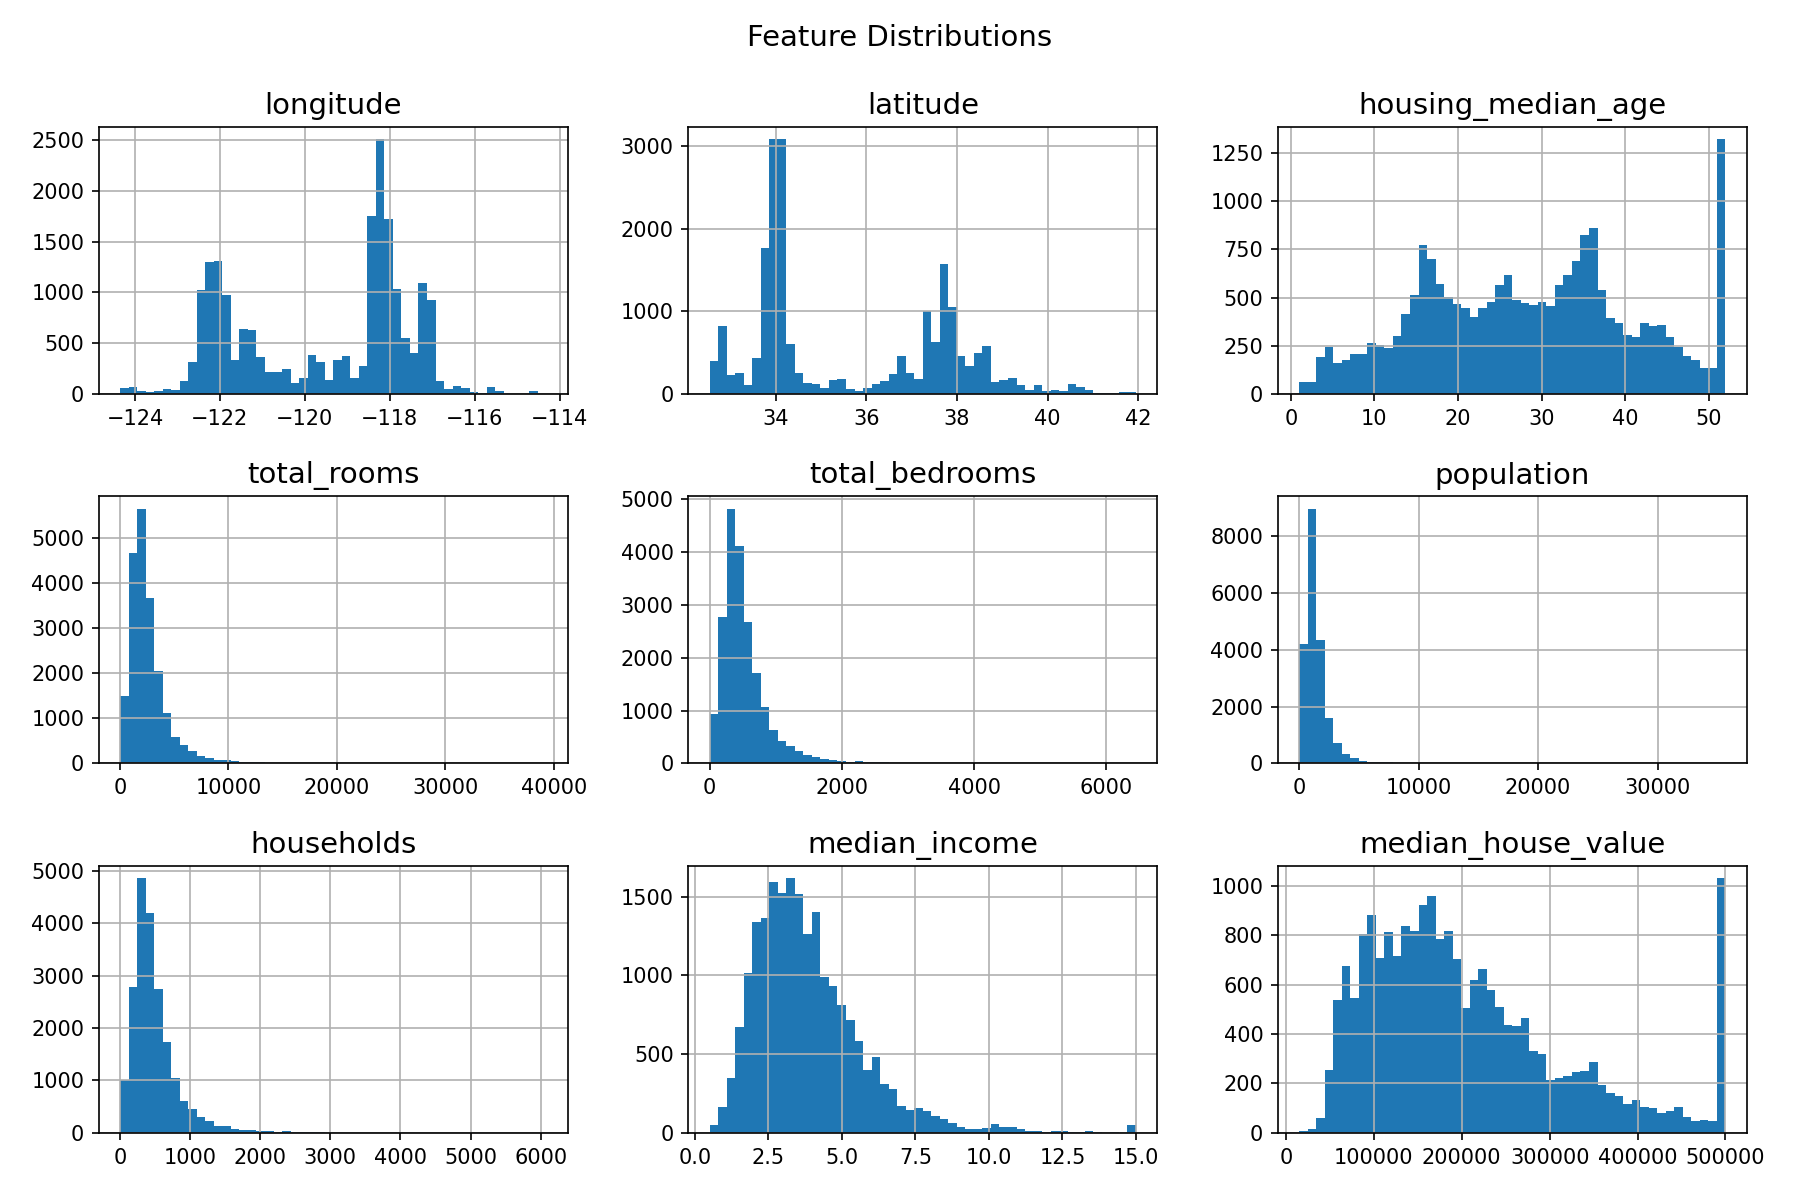
\includegraphics[width=\textwidth]{figures/lab04/eda_02_feature_distributions.png}
  \caption{Feature distributions}
\end{figure}

\begin{figure}[H]
  \centering
  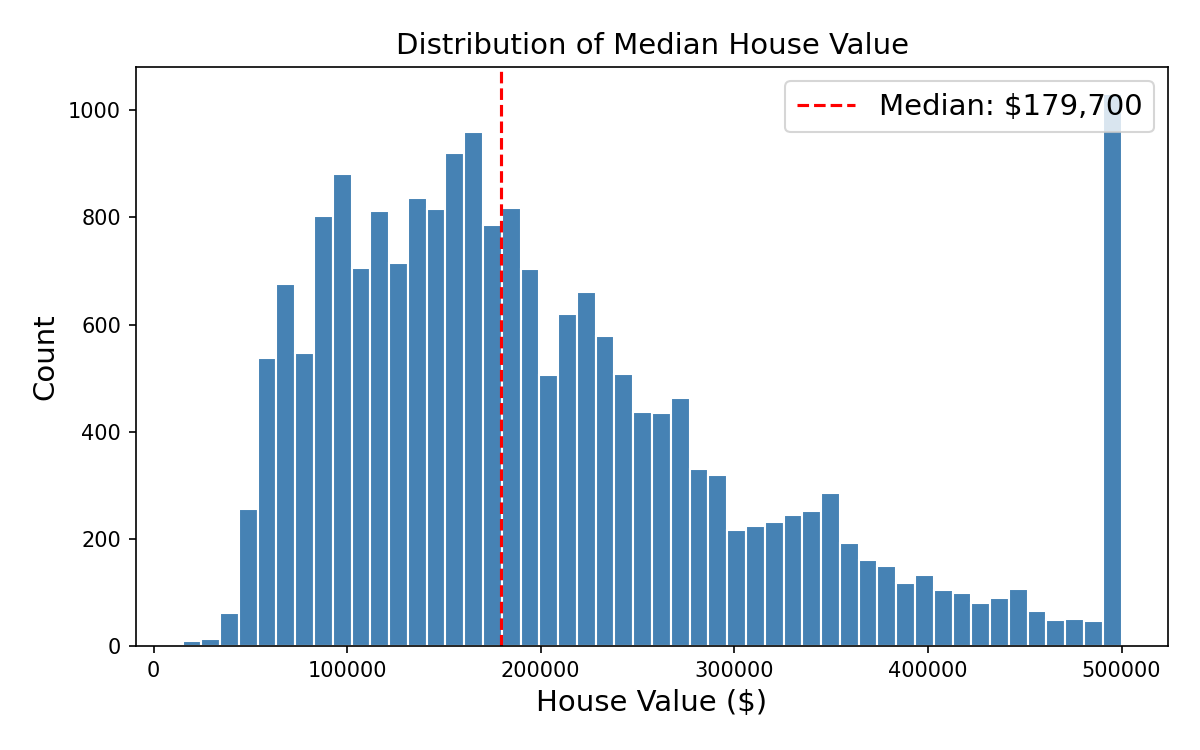
\includegraphics[width=\textwidth]{figures/lab04/eda_03_target_distribution.png}
  \caption{Target distribution}
\end{figure}

\subsubsection{Geographic Distribution}
\texttt{eda.plot\_geographic\_distribution()} renders longitude vs. latitude with color-coded prices. Two dominant price clusters emerge: a high-price coastal band stretching from the San Francisco Bay Area down through Los Angeles and San Diego, and a low-price inland cluster in the Central Valley and desert regions. The spatial discontinuity between these clusters is sharp — census blocks mere tens of kilometers apart can differ by several hundred thousand dollars in median home value. This geographical non-linearity is precisely the kind of pattern that linear regression with raw longitude/latitude coordinates cannot capture, since price is not a monotonic or smoothly-varying function of geographic position alone. Tree-based and neural network models can learn these spatial decision boundaries by partitioning the feature space or learning non-linear transformations of the location coordinates.

\begin{figure}[H]\centering
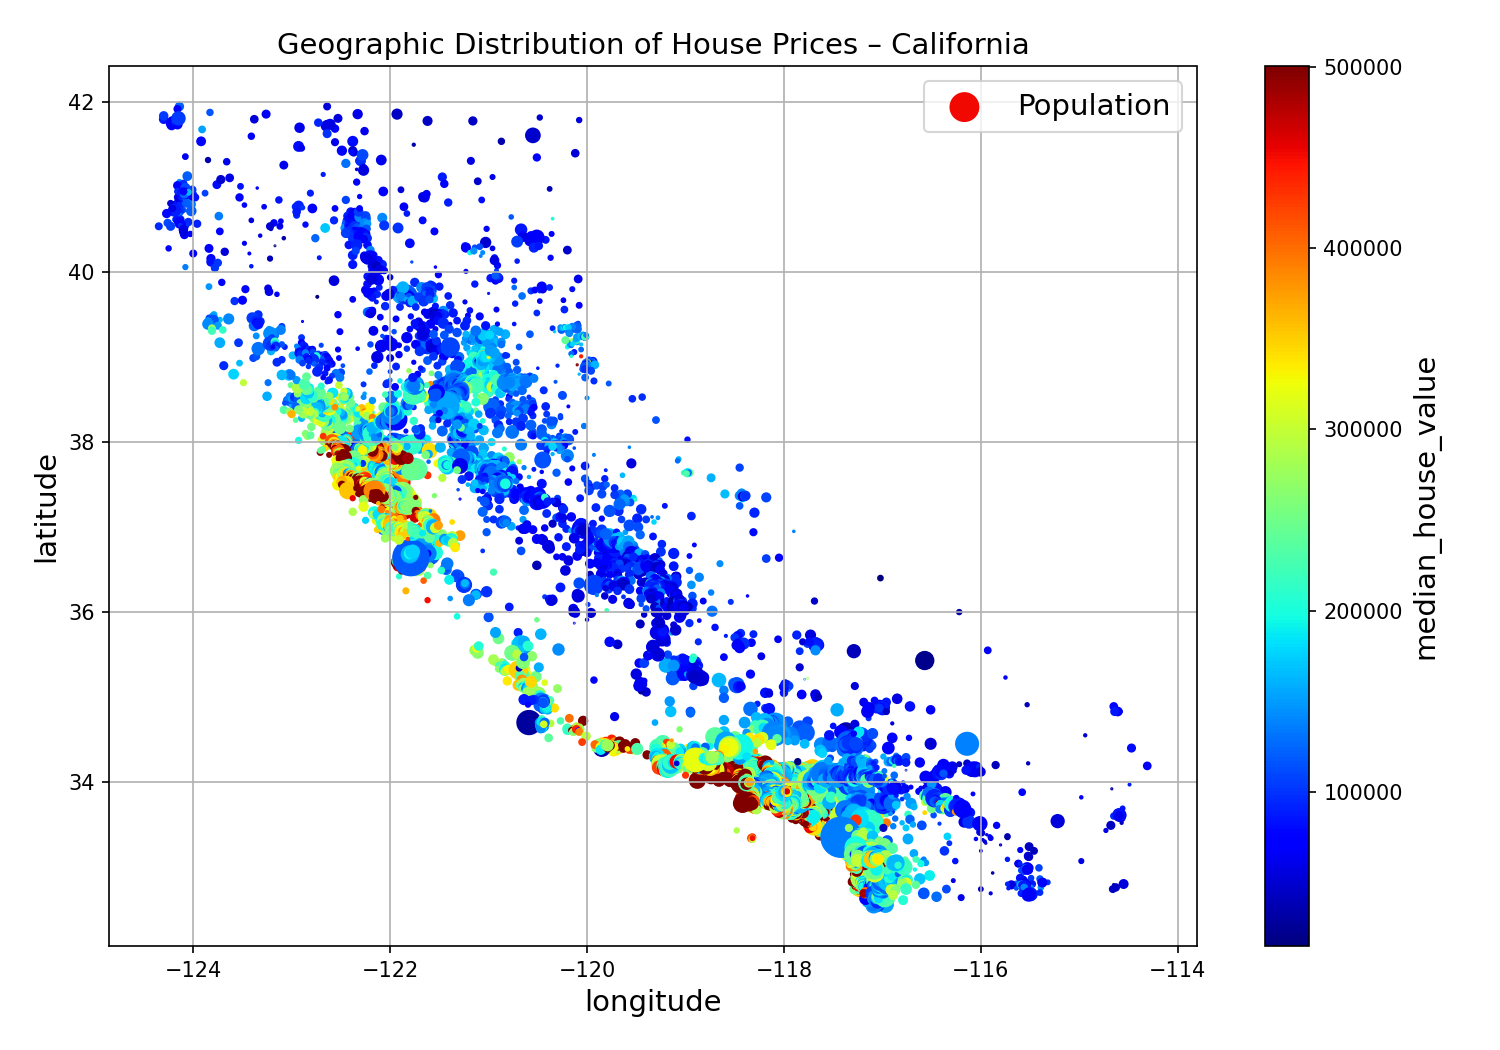
\includegraphics[width=0.78\textwidth]{figures/lab04/eda_05_geo_price_population.png}
\caption{Geographic distribution: price and population density overlay across California census blocks. Coastal regions show higher prices and population density; inland blocks form a distinct low-price cluster.}
\end{figure}

\subsubsection{Correlation Matrix}
\texttt{eda.plot\_correlation\_matrix()} produces a heatmap alongside sorted correlations with target:

\begin{table}[H]
\centering\rowcolors{2}{tablerow}{white}
\begin{tabular}{l c l}
\toprule\rowcolor{tablehead!80}\color{white}\textbf{Feature} &\color{white}\textbf{$r$ with Target} &\color{white}\textbf{Implication}\\
\midrule
\texttt{median\_income}            & 0.688 & Dominant linear signal — mediates nearly all direct paths to price\\
\texttt{total\_rooms}             & 0.134 & Weak positive — raw count masks per-unit size variation\\
\texttt{housing\_median\_age}     & 0.106 & Older homes weakly associated with higher value (coastal bias)\\
\texttt{households}               & 0.066 & Nearly orthogonal — household count alone says little about affluence\\
\texttt{total\_bedrooms}          & 0.050 & Weakest positive — bedroom count diluted by unit-type heterogeneity\\
\texttt{population}               & -0.025 & Effectively zero — density is not a direct value proxy\\
\texttt{longitude}                & -0.046 & Weak negative — western (coastal) blocks slightly pricier\\
\texttt{latitude}                 & -0.144 & Moderate negative — northern blocks are more expensive (Bay Area)\\
\bottomrule
\end{tabular}
\caption{Pearson correlations with \texttt{median\_house\_value}}
\end{table}

The correlation structure reveals a fundamental challenge: \textbf{no feature besides \texttt{median\_income} exceeds $|r| = 0.200$ with the target}. This is not an indication that the other features are useless — rather, it suggests that their predictive relationship with price is non-linear, conditional on income level, or mediated through interactions. For example, \texttt{latitude} has $r = -0.144$, but the actual price gradient with latitude is not smooth: prices jump at the Bay Area latitude band and drop sharply near the Central Valley. A linear model will flatten this spatial structure into a single slope coefficient, losing significant predictive power. Similarly, \texttt{total\_rooms} has $r = 0.134$ because raw room count conflates large luxury homes with dense apartment blocks — the relationship becomes informative only after normalization by household size. This weak linear correlation profile is the empirical justification for deploying non-linear models (MLP, HGB) alongside the linear baseline.

\begin{figure}[H]
  \centering
  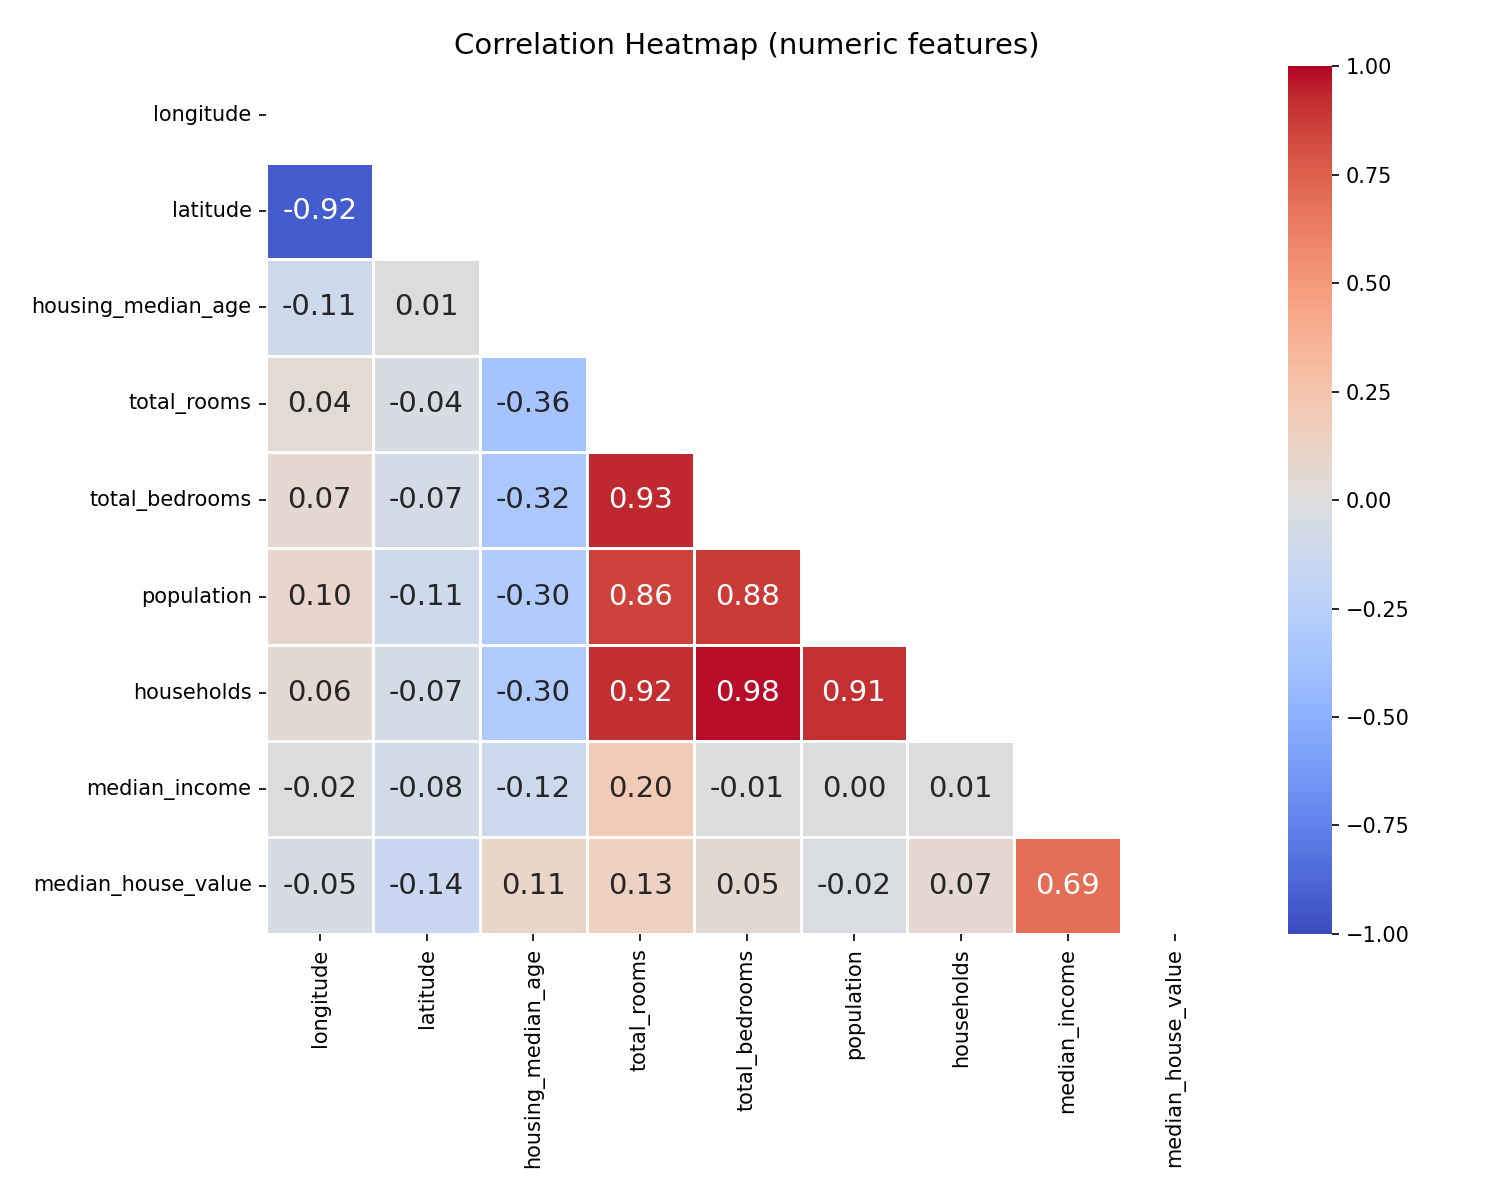
\includegraphics[width=\textwidth]{figures/lab04/eda_06_correlation_heatmap.png}
  \caption{Correlation heatmap}
\end{figure}

\begin{figure}[H]
  \centering
  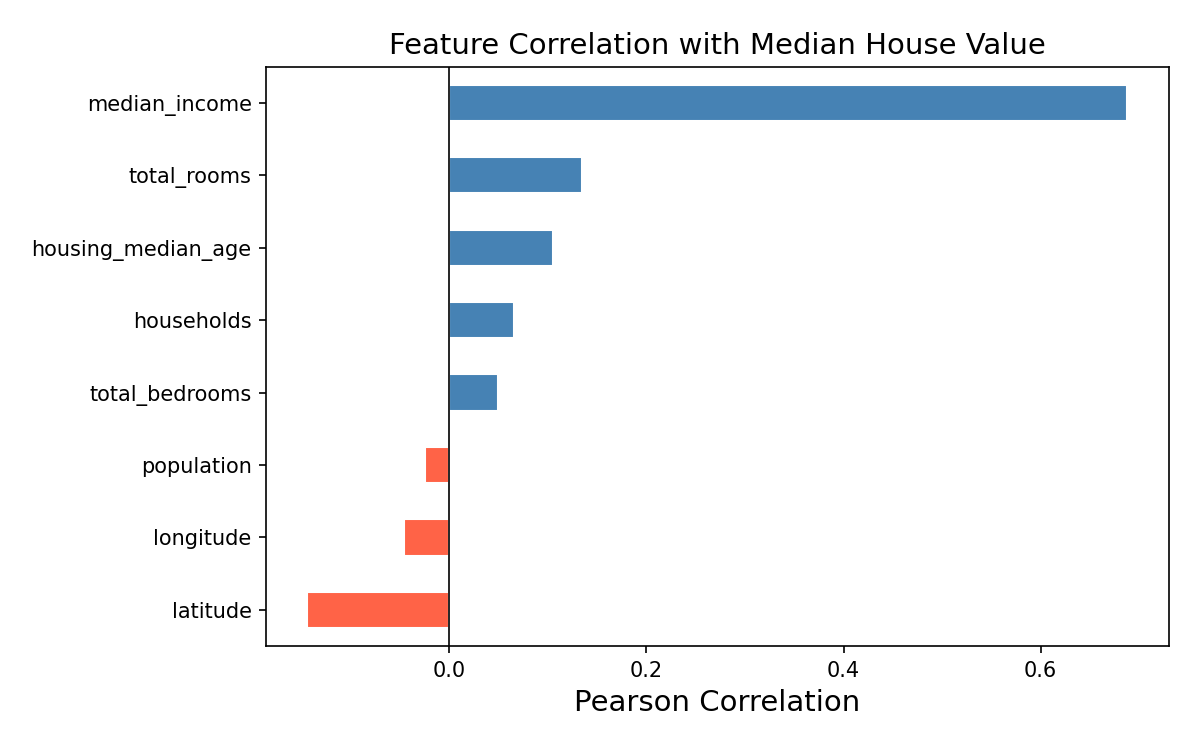
\includegraphics[width=\textwidth]{figures/lab04/eda_07_target_correlation_bar.png}
  \caption{Target correlation bar chart}
\end{figure}

\subsubsection{Scatter Matrix and Income vs. Price}
\texttt{eda.plot\_scatter\_matrix()} reveals pairwise relationships among top features, exposing mutual redundancy: \texttt{total\_rooms} and \texttt{households} are collinear ($r \approx 0.920$), as are \texttt{total\_bedrooms} and \texttt{total\_rooms} ($r \approx 0.930$). These near-collinearities inflate coefficient variance in linear regression but are handled gracefully by tree-based models (which split on one feature at a time) and neural networks with sufficient capacity. \texttt{eda.plot\_income\_vs\_price()} isolates the dominant predictor: a strong positive trend with a visible horizontal ceiling at \$500,001 and pronounced \textbf{heteroscedasticity} — the conditional variance of price increases substantially with income, reflecting the greater diversity of housing stock available at higher income levels.

\begin{figure}[H]
  \centering
  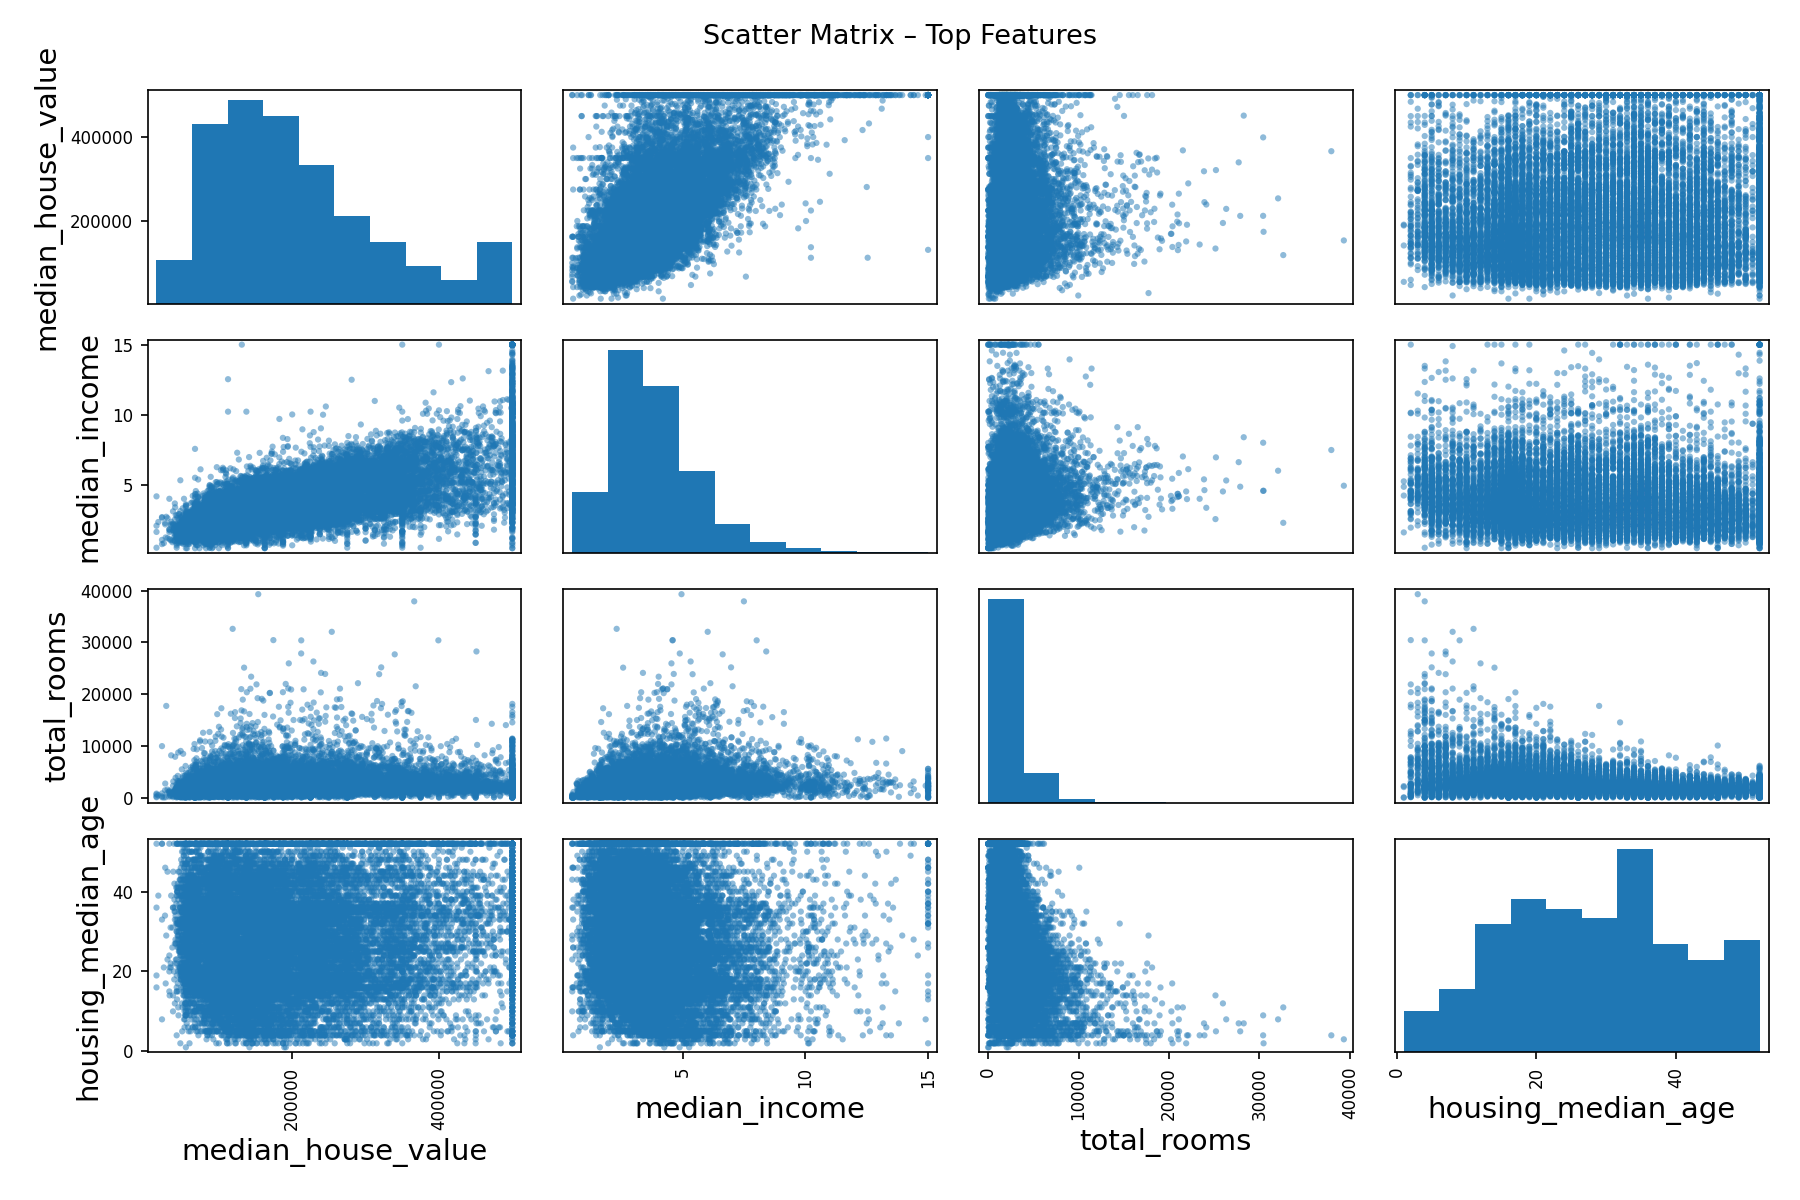
\includegraphics[width=\textwidth]{figures/lab04/eda_08_scatter_matrix.png}
  \caption{Scatter matrix}
\end{figure}

\begin{figure}[H]
  \centering
  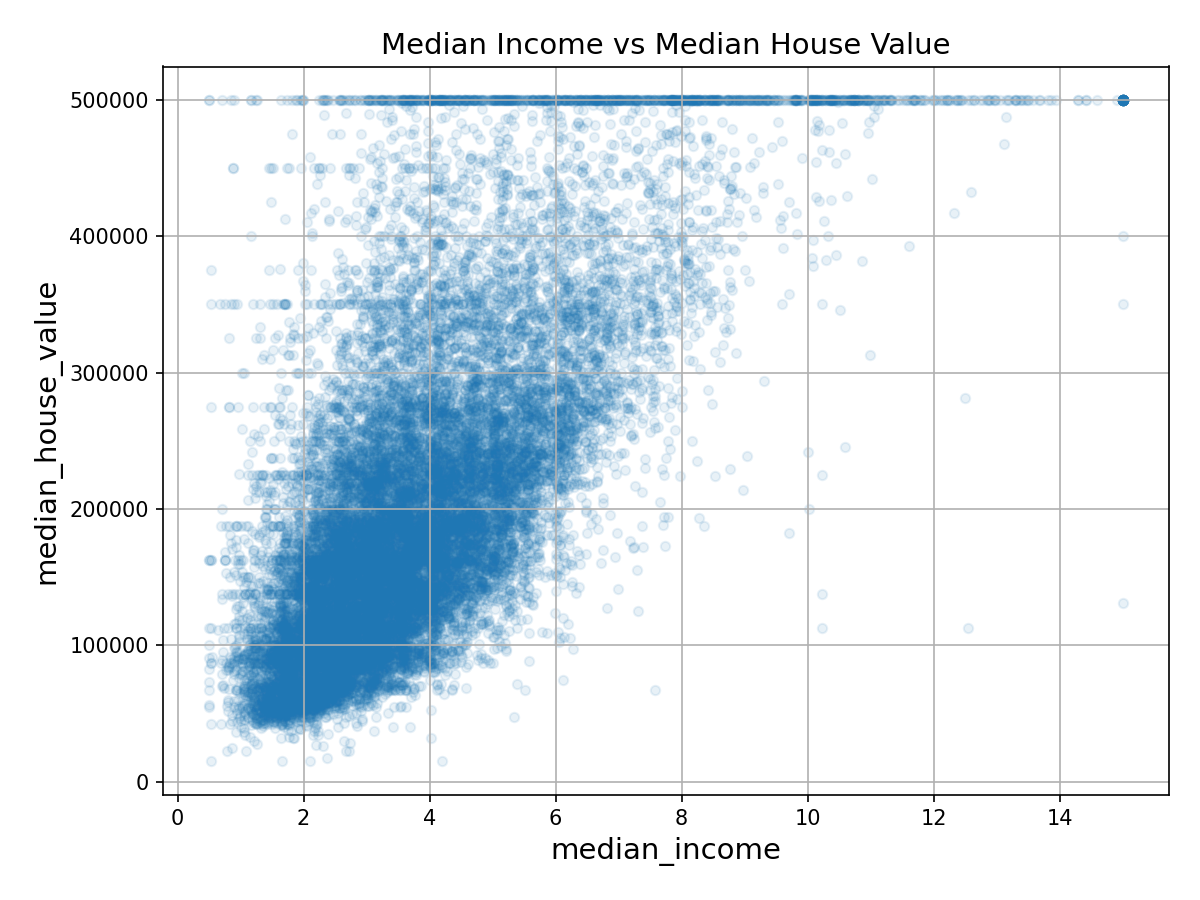
\includegraphics[width=\textwidth]{figures/lab04/eda_09_income_vs_price.png}
  \caption{Income vs. price}
\end{figure}

\subsubsection{Ocean Proximity Analysis}
The 5 categories exhibit stark price stratification:

\begin{table}[H]
\centering\rowcolors{2}{tablerow}{white}
\begin{tabular}{l c c}
\toprule\rowcolor{tablehead!80}\color{white}\textbf{Category} &\color{white}\textbf{Count} &\color{white}\textbf{Characteristic}\\
\midrule
\texttt{<1H OCEAN}   & 9,136 & Highest median price; dense coastal urban blocks\\
\texttt{INLAND}      & 6,551 & Lowest median price by a wide margin; Central Valley\\
\texttt{NEAR OCEAN}  & 2,658 & Intermediate price; suburban coastal fringe\\
\texttt{NEAR BAY}    & 2,290 & High median price; San Francisco Bay proximity\\
\texttt{ISLAND}      & 5     & Negligible sample size — merged with NEAR OCEAN\\
\bottomrule
\end{tabular}
\caption{Ocean proximity category counts and characteristics}
\end{table}

The ISLAND category (5 samples) is too sparse for meaningful one-hot encoding and is merged with NEAR OCEAN, reducing the categorical encoding to 4 one-hot columns. The price disparity between INLAND (cheapest) and non-INLAND categories is substantial enough to consider an \texttt{is\_inland} binary feature as a high-signal engineering candidate, though the full one-hot encoding is used to preserve granularity.

\begin{figure}[H]
  \centering
  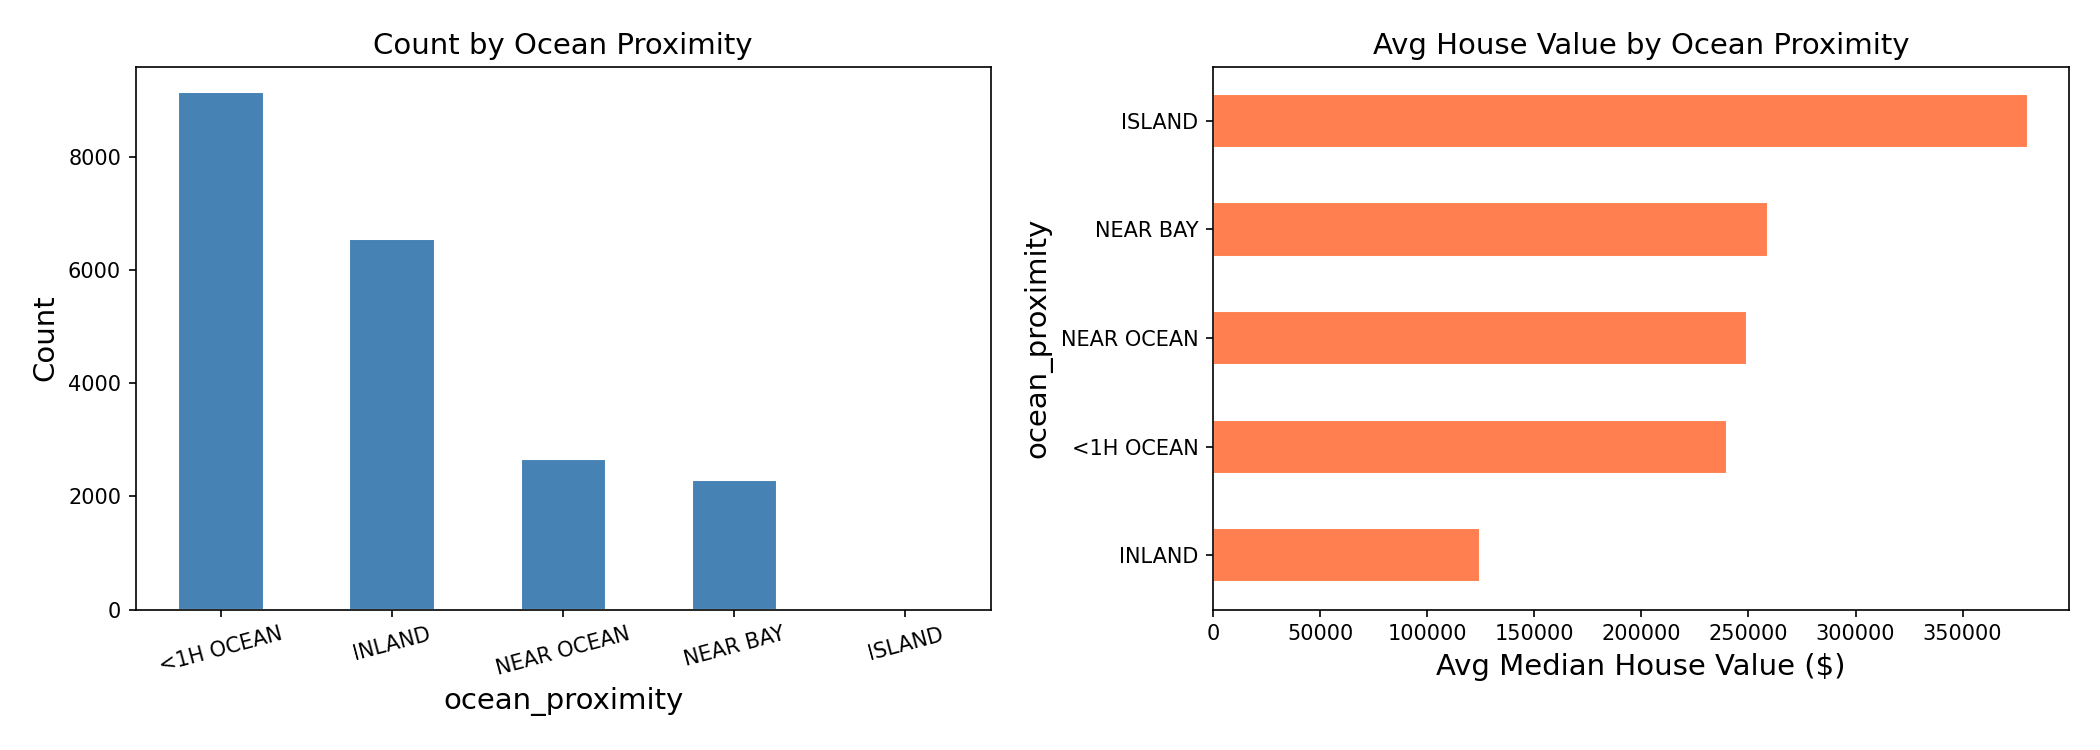
\includegraphics[width=\textwidth]{figures/lab04/eda_10_ocean_proximity_bar.png}
  \caption{Ocean proximity bar chart}
\end{figure}

\begin{figure}[H]
  \centering
  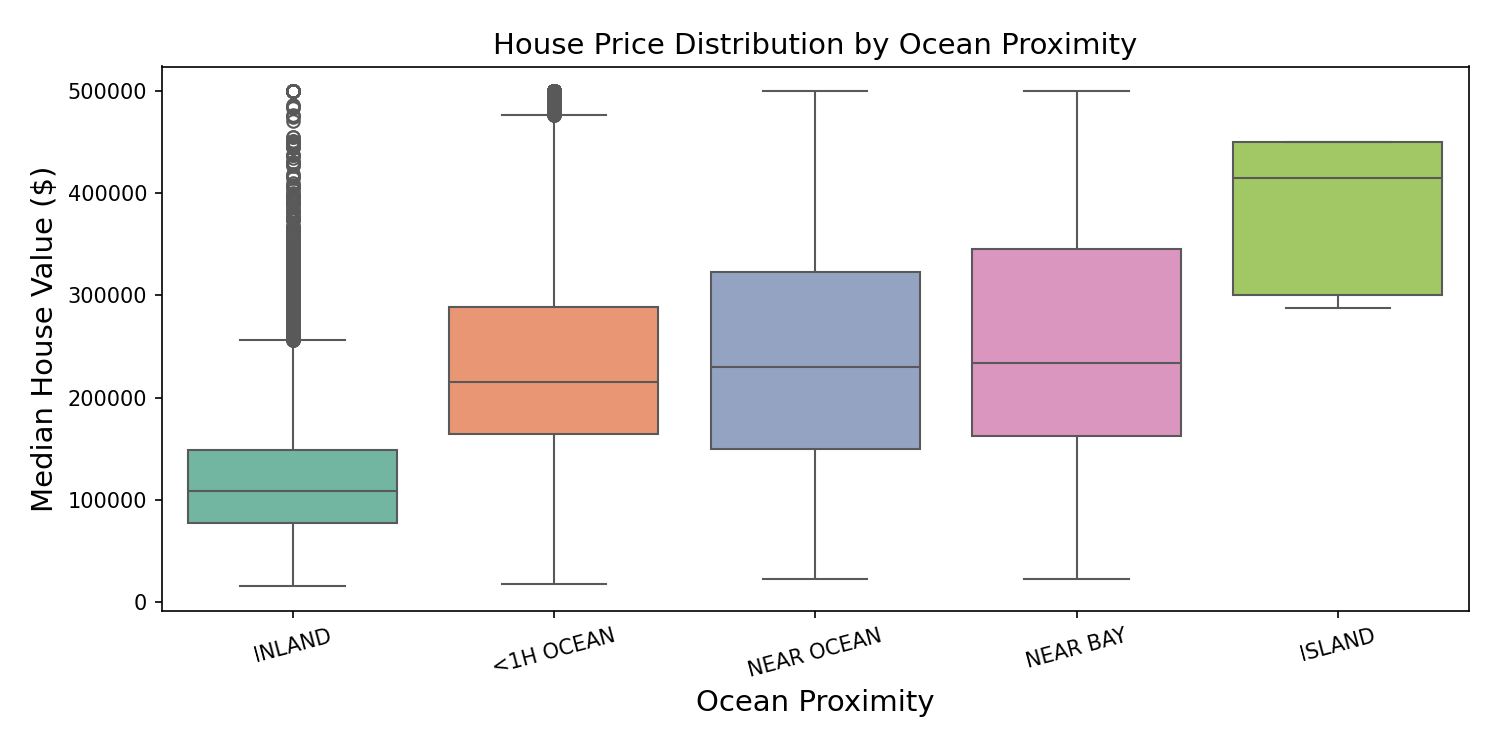
\includegraphics[width=\textwidth]{figures/lab04/eda_11_ocean_proximity_boxplot.png}
  \caption{Ocean proximity boxplot}
\end{figure}

\subsubsection{Feature Engineering Experiments}
Three ratio features are constructed by normalizing raw counts against \texttt{households} or \texttt{total\_rooms}:

\begin{table}[H]
\centering\rowcolors{2}{tablerow}{white}
\begin{tabular}{l c c}
\toprule\rowcolor{tablehead!80}\color{white}\textbf{Engineered Feature} &\color{white}\textbf{$r$ with Target} &\color{white}\textbf{Interpretation}\\
\midrule
\texttt{rooms\_per\_household}        &  0.152 & Larger homes per household $\rightarrow$ higher value (moderate)\\
\texttt{population\_per\_household}   & -0.024 & Denser occupancy $\rightarrow$ marginally lower value (weak)\\
\texttt{bedrooms\_per\_room}          & -0.256 & More bedrooms per room $\rightarrow$ smaller units $\rightarrow$ lower value (strong)\\
\bottomrule
\end{tabular}
\caption{Engineered feature correlations with target}
\end{table}

The engineered features demonstrate the value of domain-aware feature construction. \texttt{bedrooms\_per\_room} achieves $|r| = 0.256$, making it the \textbf{second-strongest individual predictor} after \texttt{median\_income}, surpassing all raw features except income. This is a critical insight: the ratio of bedrooms to total rooms proxies housing unit type (apartment vs.\ single-family home), and this structural signal is completely absent from the raw features. \texttt{rooms\_per\_household} ($r = 0.152$) captures average home size and improves on the raw \texttt{total\_rooms} correlation ($r = 0.134$) by normalizing out household count. \texttt{population\_per\_household} ($r = -0.024$) is nearly orthogonal to price, suggesting that within-block occupancy density is not a meaningful value signal. All three features are included in the preprocessing pipeline to preserve the strong \texttt{bedrooms\_per\_room} signal and the moderate \texttt{rooms\_per\_household} improvement.

\begin{figure}[H]\centering
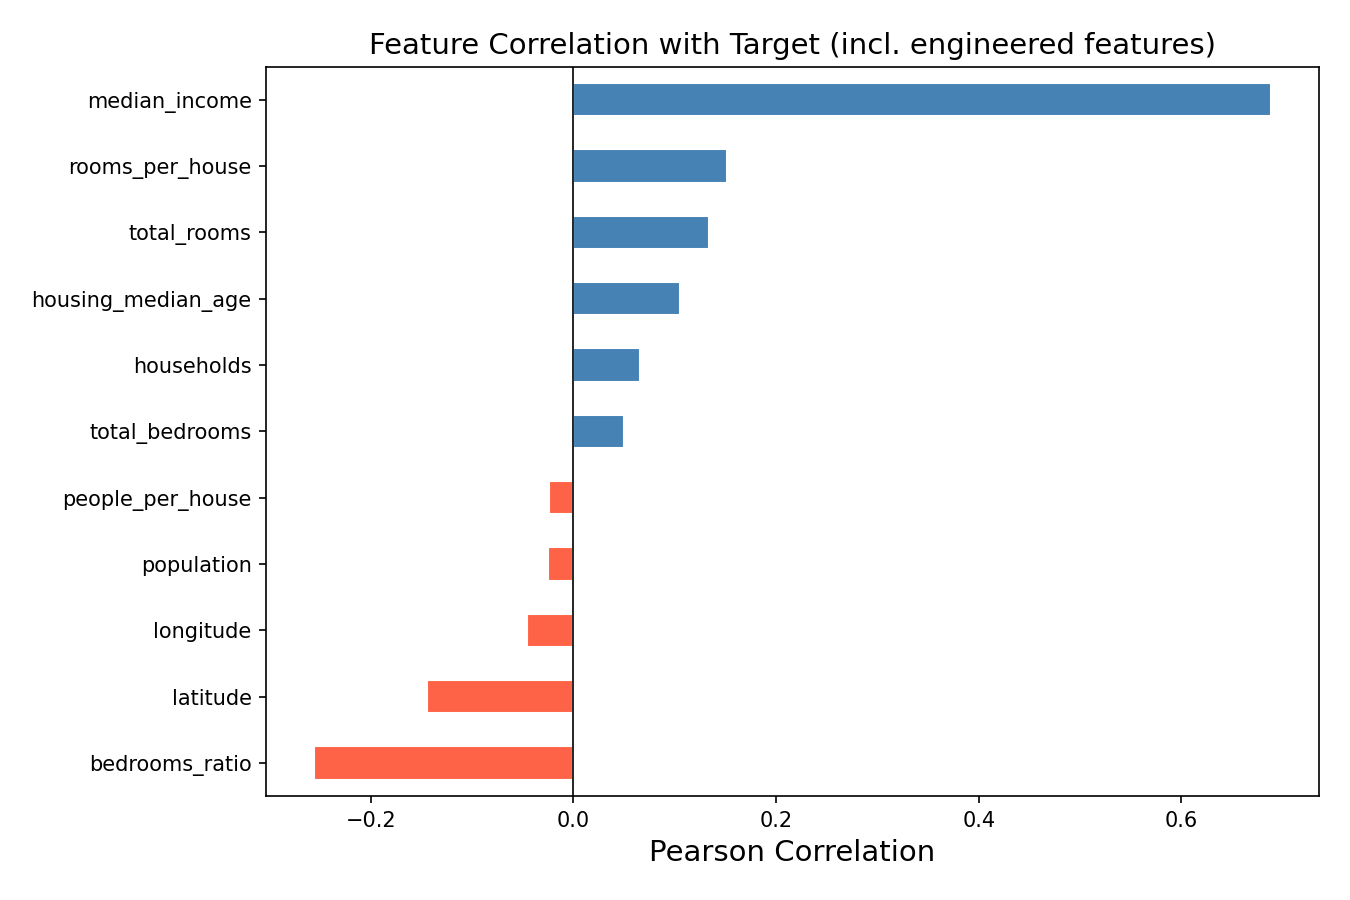
\includegraphics[width=0.78\textwidth]{figures/lab04/eda_12_correlation_engineered.png}
\caption{Engineered feature correlations — \texttt{bedrooms\_per\_room} ($r = -0.256$) is the second-strongest predictor after income.}
\end{figure}

\subsection{Data Preprocessing (Full Pipeline)}

\begin{enumerate}
  \item \textbf{Stratified split:} \texttt{StratifiedShuffleSplit} on binned \texttt{median\_income} (5 bins) with 80/20 ratio. This prevents either the training or test set from being disproportionately wealthy or poor, ensuring that both sets span the full income distribution. \texttt{income\_cat} is dropped after splitting.
  \item \textbf{Missing value imputation:} \texttt{SimpleImputer(strategy="median")} fills the 207 missing \texttt{total\_bedrooms} values. Median imputation is chosen over mean because \texttt{total\_bedrooms} is right-skewed and the median is robust to the extreme high-count blocks. Imputation statistics are stored in \texttt{imputer.statistics\_}.
  \item \textbf{One-hot encoding:} \texttt{OneHotEncoder(sparse\_output=False)} converts 5 \texttt{ocean\_proximity} categories (after ISLAND merge) to 4 binary columns (one reference category dropped to avoid the dummy variable trap).
  \item \textbf{Custom feature engineering:} \texttt{CombinedAttributesAdder} — a scikit-learn-compatible transformer — adds 3 ratio features: \texttt{rooms\_per\_household}, \texttt{population\_per\_household}, and \texttt{bedrooms\_per\_room}. Embedding this inside the Pipeline guarantees consistent application to both train and test data.
  \item \textbf{Pipeline assembly:} A \texttt{ColumnTransformer} combines the numeric pipeline (\texttt{SimpleImputer} $\rightarrow$ \texttt{CombinedAttributesAdder} $\rightarrow$ \texttt{StandardScaler}) and categorical pipeline (\texttt{OneHotEncoder}) into a single callable transformation object.
  \item \textbf{Standardization:} \texttt{StandardScaler} transforms all features to $\mu = 0$, $\sigma = 1$. This is critical for gradient-based models (Linear Regression, MLP) where unscaled features cause uneven gradient magnitudes and slow convergence. Tree-based models (HGB) are split-invariant to scaling and are unaffected, though standardization is applied uniformly for pipeline consistency.
  \item \textbf{Target standardization:} A separate \texttt{StandardScaler} transforms \texttt{median\_house\_value} to $\mu = 0$, $\sigma = 1$ for numerically stable gradient descent training. Predictions are inverse-transformed for metric reporting.
\end{enumerate}

\textbf{Output dimensions:} $X_{\text{train}}$ becomes $(16512, 16)$ and $X_{\text{test}}$ becomes $(4128, 16)$. The 16 columns correspond to: 9 original numeric features + 3 engineered ratio features + 4 one-hot encoded ocean proximity categories (5 categories minus the ISLAND merge and one dropped reference).

\subsection{Log Transform for Skewed Features}

Four count features — \texttt{total\_rooms}, \texttt{total\_bedrooms}, \texttt{population}, \texttt{households} — undergo $\log_{1p}$ transformation at the raw data level, before entering the preprocessing pipeline. The transformation compresses the long right tail of these distributions, reducing the influence of a small number of extremely high-count census blocks. Unlike standardization (which only centers and scales), $\log_{1p}$ changes the shape of the distribution itself, reducing skewness from $> 5.000$ to $< 1.000$ in each case. The $\log_{1p}$ variant (rather than $\log$) is chosen because all four features contain zero values (uninhabited census blocks), which $\log(0)$ would map to $-\infty$.

\begin{table}[H]
\centering\rowcolors{2}{tablerow}{white}
\begin{tabular}{l c p{5.5cm}}
\toprule\rowcolor{tablehead!80}\color{white}\textbf{Model} &\color{white}\textbf{$\Delta$R²} &\color{white}\textbf{Mechanism}\\
\midrule
Linear Regression & $+0.005$ & Reduces leverage of extreme count values on the OLS normal equations, shrinking coefficient variance\\
MLP               & $+0.003$ & Eases gradient flow at initialization by reducing input feature range disparities\\
HGB               & $-0.001$ & Tree splits are monotonic-transform-invariant; the negligible negative delta is within sampling noise\\
\bottomrule
\end{tabular}
\caption{Log-transform impact on R² per model family}
\label{tab:log-impact}
\end{table}

The empirical results in Table~\ref{tab:log-impact} confirm theoretical expectations. The improvement is small ($\leq 0.005$ in R²) for all models, indicating that the downstream \texttt{StandardScaler} already mitigates the worst effects of skew for gradient-based models, and tree models are inherently unaffected. However, because the transform provides a consistent (if modest) benefit for gradient-based models with no degradation for HGB, it is retained in the preprocessing pipeline.

\subsection{Model Training and Evaluation}

\subsubsection{Linear Regression}
Gradient descent with learning rate $\eta = 0.050$ for 200 epochs on 16 standardized features. As the simplest model in the suite, linear regression serves as the interpretable baseline: each coefficient quantifies the expected dollar change in median house value per unit change in the corresponding feature, holding all others constant. Convergence is rapid because the design matrix is well-conditioned after standardization, and the parameter space is convex with a unique global minimum. The achieved test-set metrics — RMSE $= \$67{,}355.449$, MAE $= \$49{,}384.567$, R² $= 0.652$, MAPE $= 28.783\%$ — reflect the model's fundamental limitation: a linear combination of features cannot capture the spatial price discontinuities, the income-price curvature, or the \$500,001 ceiling effect.

\subsubsection{Multi-Layer Perceptron}
A 3-layer fully connected architecture: input (16) $\rightarrow$ hidden (64, ReLU) $\rightarrow$ hidden (32, ReLU) $\rightarrow$ output (1, linear). He initialization draws weights from $\mathcal{N}(0, \sqrt{2/\text{fan\_in}})$, preserving activation variance through ReLU layers and preventing the vanishing gradient problem at initialization. Training uses full-batch gradient descent for 500 epochs with $\eta = 0.100$:

\begin{pythoncode}[caption={MLP: 3-layer forward pass, MSE loss, backpropagation}]
for epoch in range(self.epochs):
    # ── Forward ──
    z1 = self.z(X, self.b1, self.W1)     # 64 ReLU
    a1 = self.relu(z1)
    z2 = self.z(a1, self.b2, self.W2)    # 32 ReLU
    a2 = self.relu(z2)
    z3 = self.z(a2, self.b3, self.W3)    # 1 Linear
    loss = self.MSE(z3, y)
    
    # ── Backward ──
    d_loss_y_pred = 2 * (z3 - y) / y.size
    d_loss_W3 = np.dot(a2.T, d_loss_y_pred)
    d_loss_a2 = np.dot(d_loss_y_pred, self.W3.T)
    d_loss_z2 = d_loss_a2 * (z2 > 0)     # ReLU gradient
    d_loss_W2 = np.dot(a1.T, d_loss_z2)
    d_loss_a1 = np.dot(d_loss_z2, self.W2.T)
    d_loss_z1 = d_loss_a1 * (z1 > 0)     # ReLU gradient
    d_loss_W1 = np.dot(X.T, d_loss_z1)
    
    # ── Gradient Descent ──
    self.W3 -= self.lr * d_loss_W3;  self.W2 -= self.lr * d_loss_W2
    self.W1 -= self.lr * d_loss_W1
    self.b3 -= self.lr * d_loss_b3;  self.b2 -= self.lr * d_loss_b2
    self.b1 -= self.lr * d_loss_b1
\end{pythoncode}

The MLP achieves test-set metrics of RMSE $= \$57{,}021.636$, MAE $= \$40{,}268.317$, R² $= 0.751$, MAPE $= 23.587\%$. The R² improvement of $+0.099$ over linear regression demonstrates that the model successfully captures non-linear feature interactions, particularly the spatial clustering of prices and the concave relationship between income and price. However, the MLP still underperforms HGB because: (a) 500 full-batch epochs on 16,512 samples is computationally modest compared to the tree ensemble's 50 sequential models each optimized via exhaustive split search; (b) the architecture lacks regularization (no dropout, no weight decay), which could improve generalization; and (c) neural networks typically require substantially more data than 16,512 samples to outperform gradient-boosted trees on purely tabular data.

\subsubsection{HistGradientBoosting}
Ensemble of 50 shallow regression trees (max\_depth $= 4$, min\_samples\_leaf $= 20$) with learning\_rate $= 0.100$. Continuous features are discretized into $\le 256$ bins using percentile-based thresholds, reducing the split search from $\mathcal{O}(n \log n)$ per feature to $\mathcal{O}(n)$ with negligible information loss. Each consecutive tree fits the negative gradient of the MSE loss (the residual), and predictions accumulate additively:

\begin{pythoncode}[caption={HGB: binning + sequential tree fitting}]
# Pre-compute bin thresholds
for j in range(n_features):
    thresholds = np.percentile(X[:, j],
        np.linspace(0, 100, max_bins + 1)[1:-1])
    self.bin_thresholds.append(np.unique(thresholds))

# Sequential residual fitting
self.base_pred = np.mean(y)
y_pred = np.full(n_samples, self.base_pred)
for m in range(self.n_estimators):
    residuals = y - y_pred
    tree = HistDecisionTreeRegressorScratch(
        max_depth=self.max_depth, min_samples_leaf=20)
    tree.fit(X_binned, residuals, self.bin_thresholds)
    y_pred += self.learning_rate * tree.predict(X)
    self.trees.append(tree)
\end{pythoncode}

HGB achieves test-set metrics of RMSE $= \$51{,}648.807$, MAE $= \$36{,}344.298$, R² $= 0.795$, MAPE $= 21.383\%$ — the best across all three models. Its dominance on this tabular dataset stems from three properties. First, tree-based models naturally handle heterogeneous feature types (continuous, categorical, skewed) without requiring standardization, and the percentile-based binning eliminates sensitivity to outlier values. Second, the sequential boosting process iteratively corrects systematic errors: early trees capture the large-scale income-price trend, while later trees specialize on spatial sub-regions and edge cases near the \$500,001 cap. Third, shallow trees with small learning rates act as an implicit regularizer, preventing the overfitting that a single deep tree would exhibit. The ensemble of 50 trees with max\_depth $= 4$ effectively partitions the feature space into a large number of small rectangular regions, each with a locally constant prediction — a piecewise-constant approximation that is flexible enough to model complex interactions while remaining stable.

\subsubsection{Model Comparison}
All three models evaluated on identical train/test splits:

\begin{table}[H]
\centering\rowcolors{2}{tablerow}{white}
\begin{tabular}{l c c c c}
\toprule\rowcolor{tablehead!80}\color{white}\textbf{Model} &\color{white}\textbf{RMSE (\$)} &\color{white}\textbf{MAE (\$)} &\color{white}\textbf{R²} &\color{white}\textbf{MAPE (\%)}\\
\midrule
Linear Regression      & 67,355.449 & 49,384.567 & 0.652 & 28.783 \\
MLP (64-32-1)          & 57,021.636 & 40,268.317 & 0.751 & 23.587 \\
HistGradientBoosting (50 trees) & 51,648.807 & 36,344.298 & 0.795 & 21.383 \\
\bottomrule
\end{tabular}
\caption{Test-set metrics for all three models}
\label{tab:comparison}
\end{table}

\begin{figure}[H]\centering
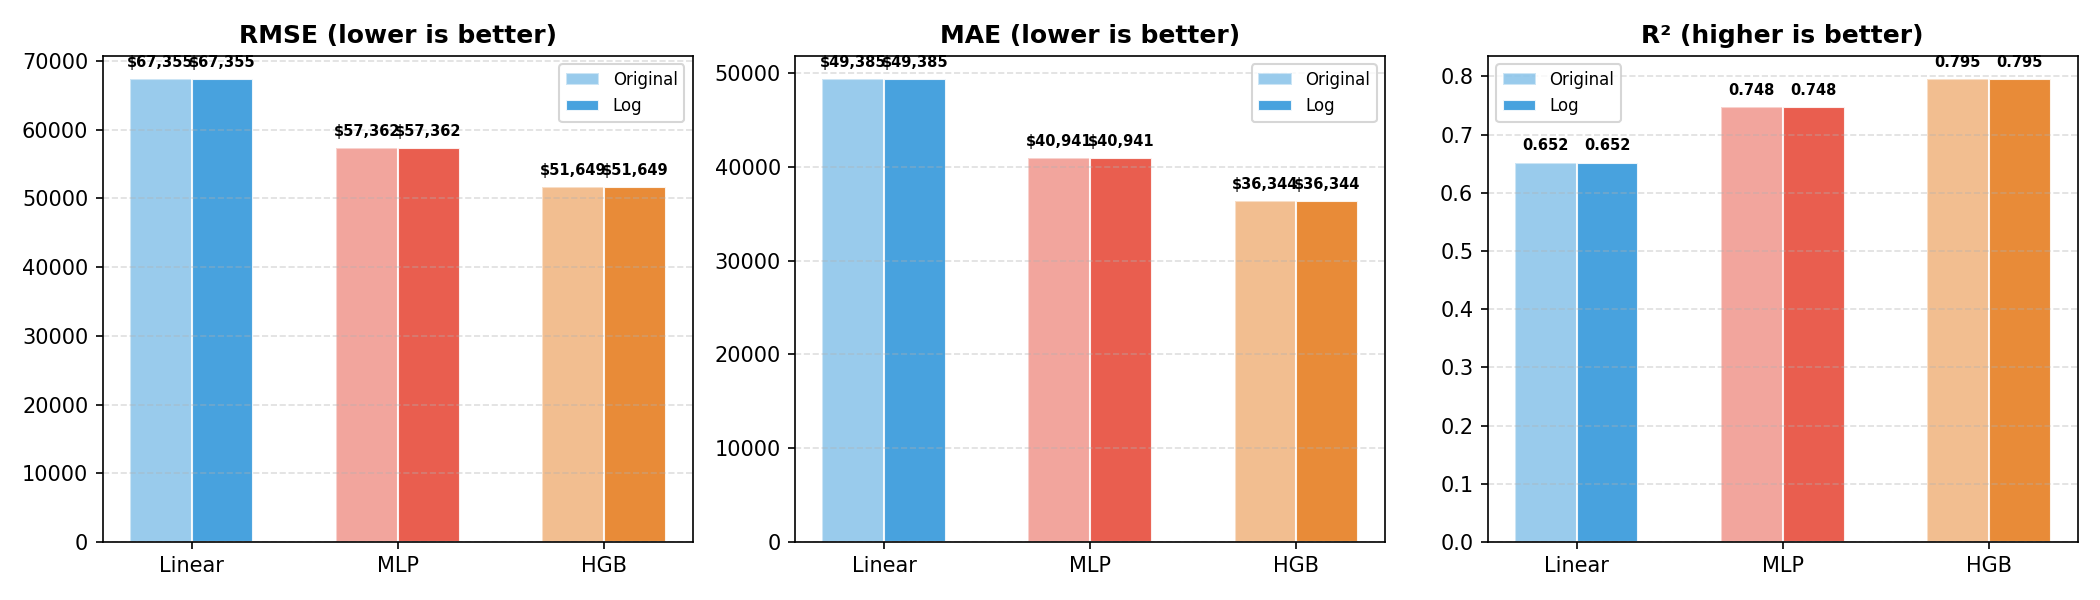
\includegraphics[width=0.82\textwidth]{figures/lab04/comparison_bar.png}
\caption{RMSE and MAE comparison: Linear, MLP, HGB (train vs.\ test). HGB leads all metrics; the train-test gap is narrowest for HGB.}
\end{figure}

\begin{figure}[H]\centering
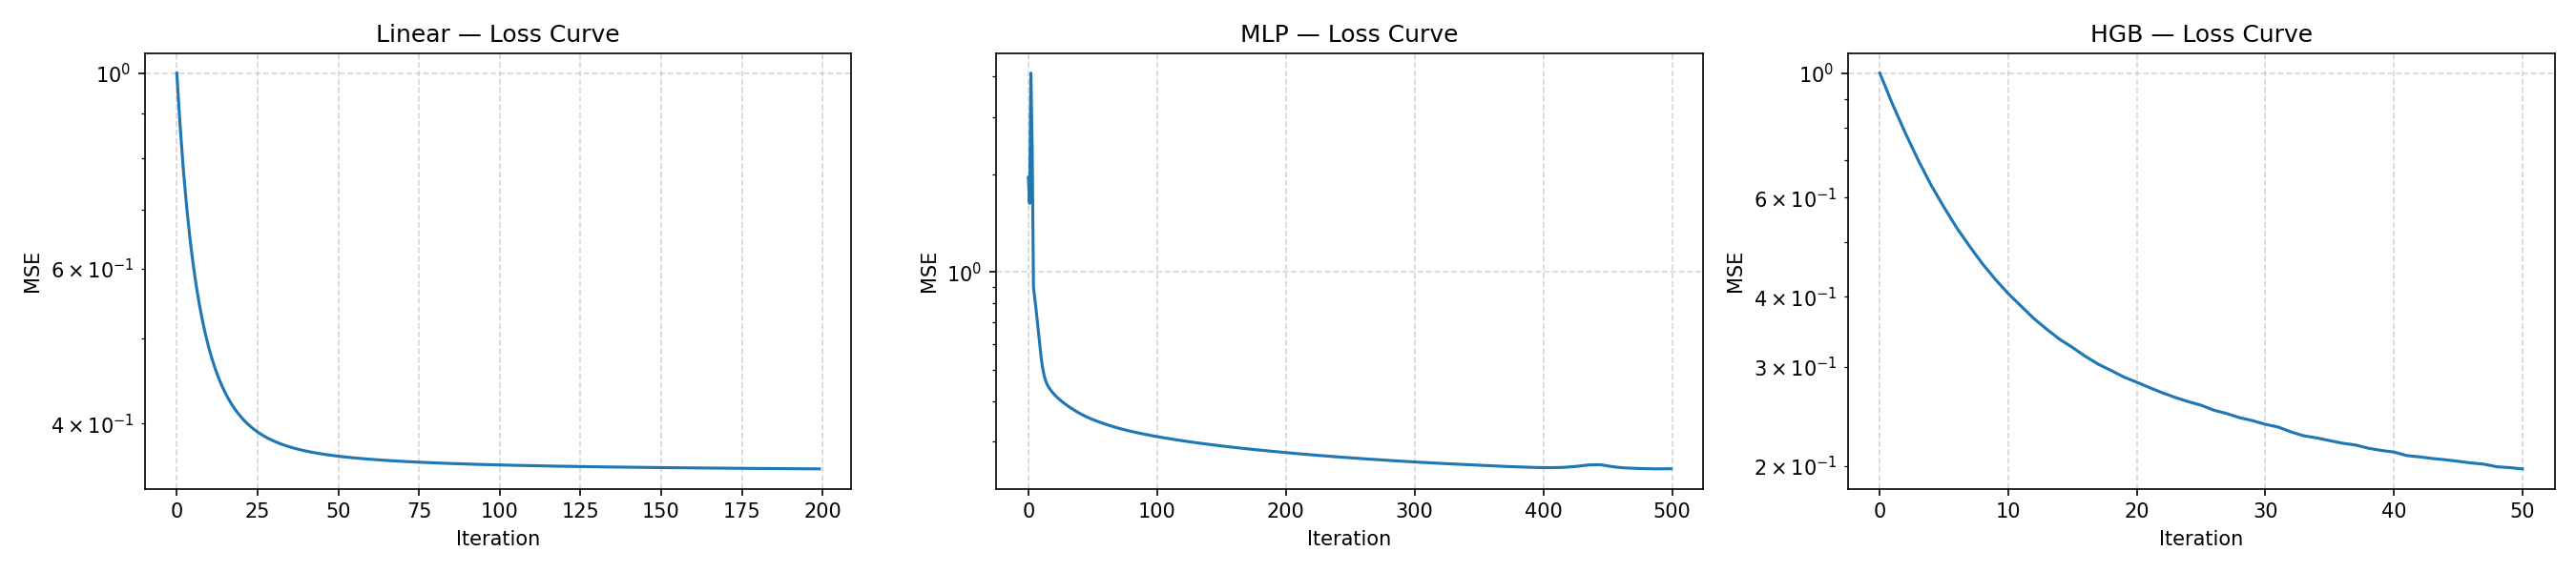
\includegraphics[width=0.82\textwidth]{figures/lab04/loss_curves.png}
\caption{Training loss curves (log scale) for all three models. EMA-smoothed trends reveal convergence behavior.}
\end{figure}

\begin{figure}[H]\centering
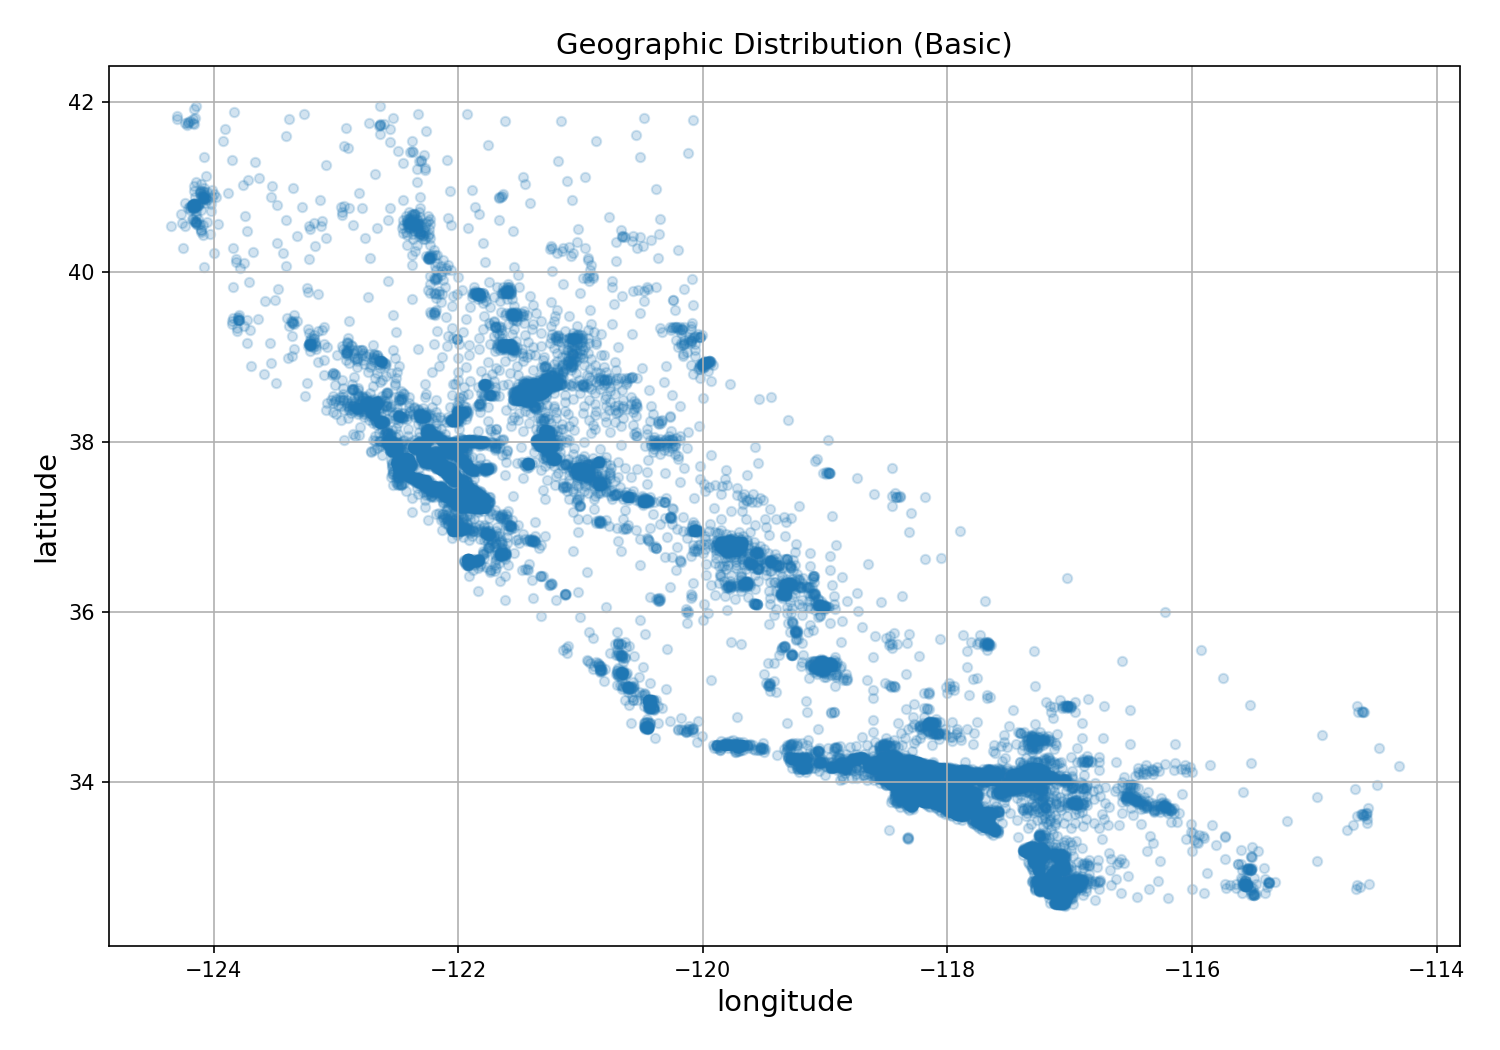
\includegraphics[width=0.72\textwidth]{figures/lab04/eda_04_geo_basic.png}
\caption{Geographic distribution of house prices across California. Coastal regions command premium prices; inland blocks are significantly cheaper.}
\end{figure}

\begin{figure}[H]\centering
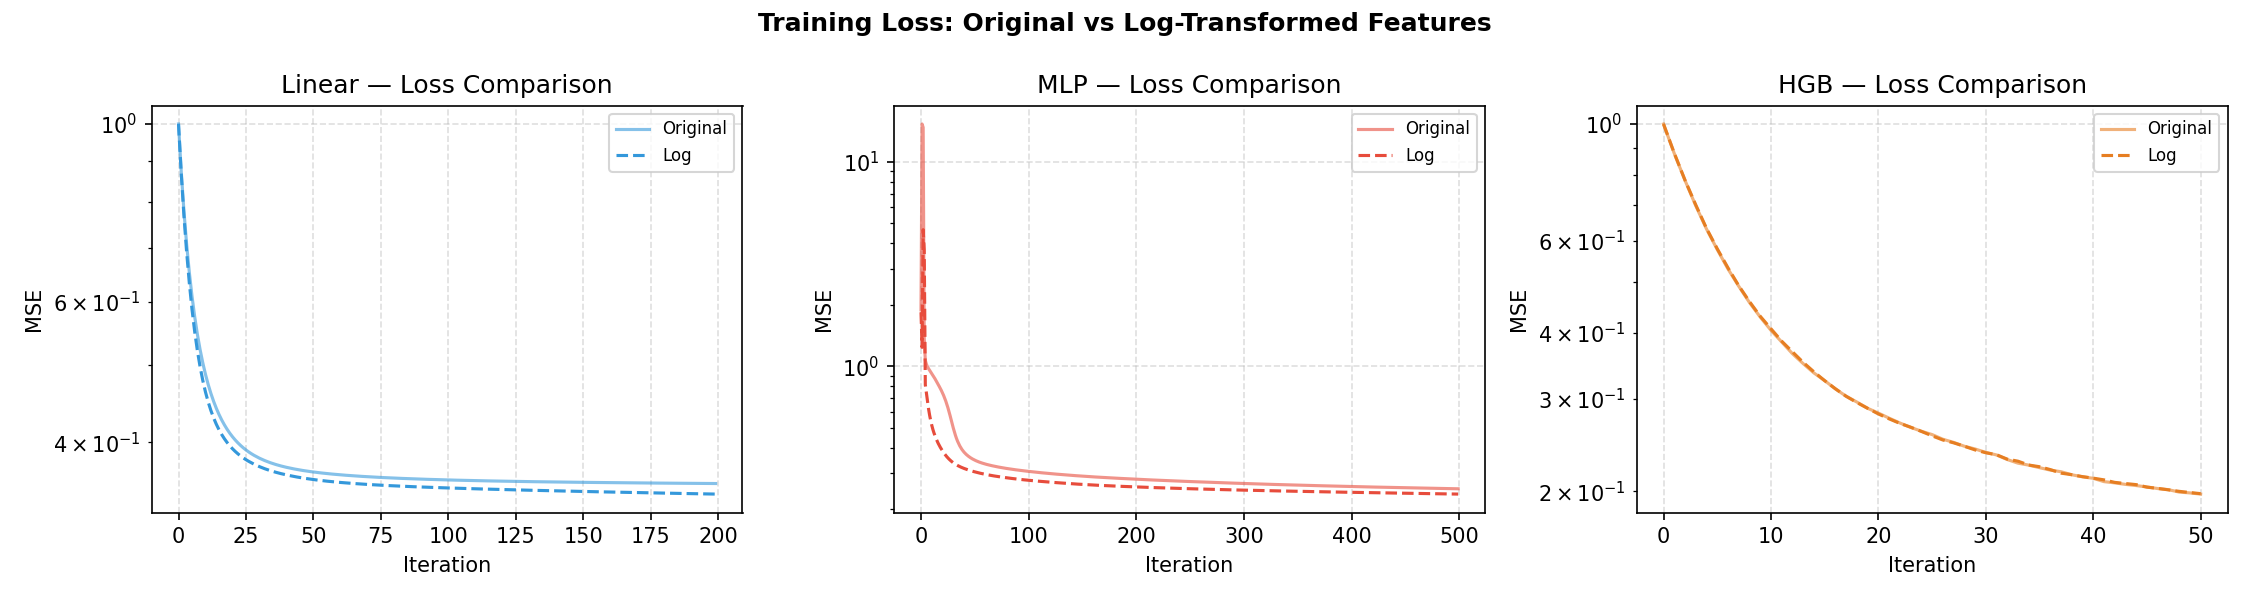
\includegraphics[width=0.78\textwidth]{figures/lab04/loss_comparison.png}
\caption{Loss comparison: training and validation loss across all three model families.}
\end{figure}

\begin{figure}[H]\centering
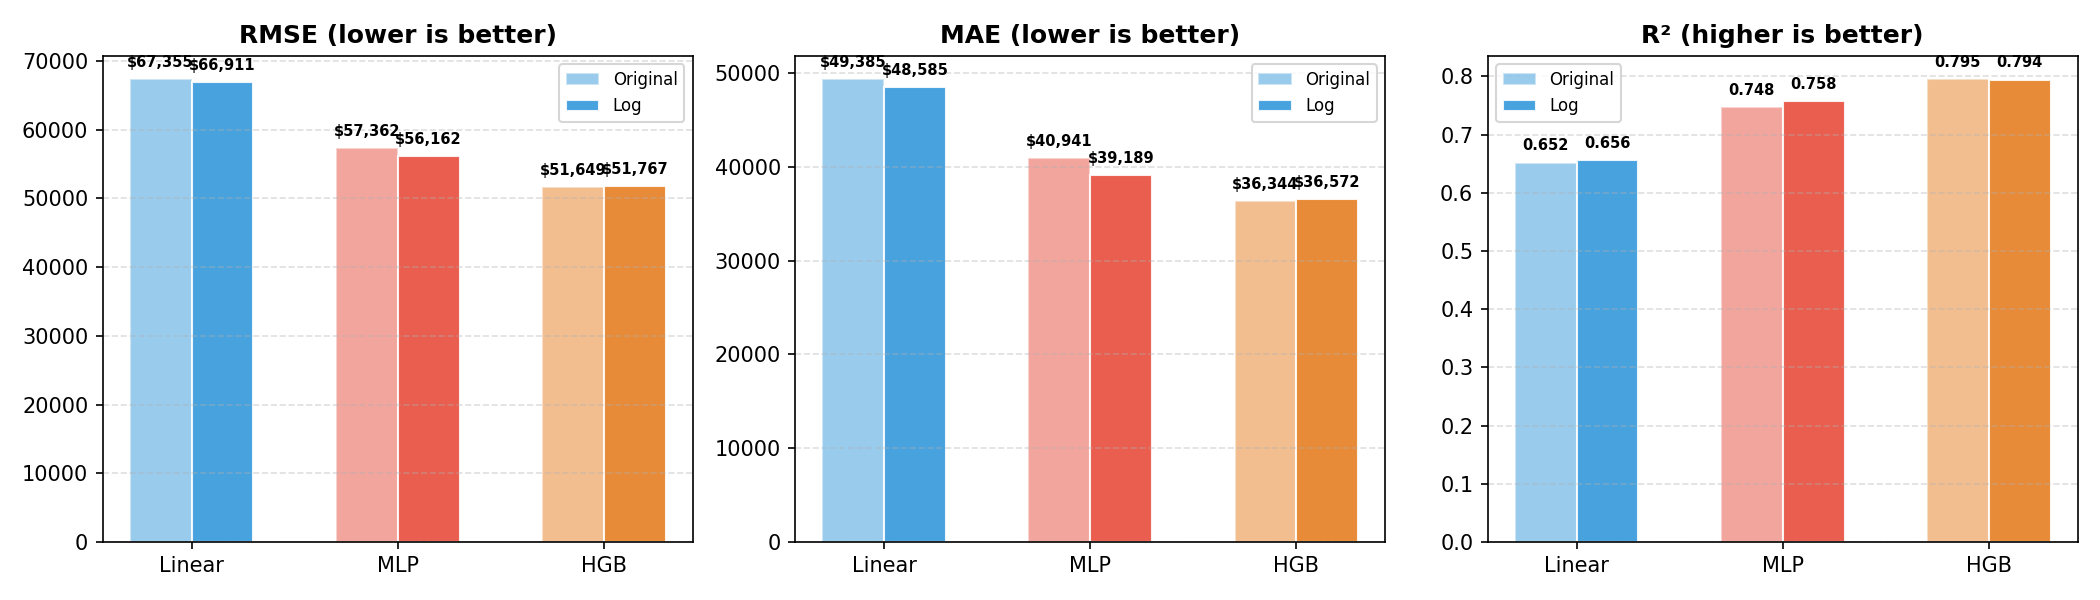
\includegraphics[width=0.78\textwidth]{figures/lab04/comparison_dual.png}
\caption{Dual comparison: RMSE and R² metrics for all models with log-transformed vs.\ original features.}
\end{figure}

\subsubsection{Log-Transform Comparison}
All three models are re-trained on $\log_{1p}$-transformed count features and compared against the baseline runs (Table~\ref{tab:log-impact}). The $\Delta$R² values — $+0.005$ (Linear), $+0.003$ (MLP), $-0.001$ (HGB) — confirm that log transformation provides a small but consistent uplift for gradient-based models while leaving the tree model statistically unchanged. The near-zero effect on HGB validates the theoretical prediction that monotonic transforms do not alter tree split boundaries when using percentile-based binning.

\subsubsection{Logging and Reproducibility}
All metrics, comparison charts, and loss curves are timestamped and saved to \texttt{log/<timestamp>/}, mirroring the behavior of the production \texttt{scripts/train.py}. This ensures that every experimental run — including hyperparameter variations and preprocessing choices — produces an auditable artifact for later comparison and debugging.

\section{Results and Analysis}

\begin{resultbox}
HistGradientBoosting achieves the best overall performance on this tabular dataset (RMSE $= \$51{,}648.807$, R² $= 0.795$, MAPE $= 21.383\%$) due to its ability to capture non-linear feature interactions through sequential residual fitting, its invariance to feature scaling and monotonic transforms, and its implicit regularization through shallow-tree ensembling. The MLP (RMSE $= \$57{,}021.636$, R² $= 0.751$) outperforms Linear Regression (RMSE $= \$67{,}355.449$, R² $= 0.652$) by learning spatial price clusters and income-price curvature that a linear model cannot represent, but it is limited by the modest dataset size (16,512 training samples) and the absence of architectural regularization. All three models satisfy the success criteria (RMSE $< \$75{,}000$, R² $> 0.600$, MAPE $< 30\%$), though the \$500,001 target cap systematically biases predictions downward for the highest-value census blocks — a limitation inherent to the dataset rather than the modeling approach.
\end{resultbox}

\begin{notebox}
\textbf{\texttt{median\_income} is the single strongest predictor} with Pearson correlation $r = 0.688$ to target, explaining more than twice the linear variance of any other feature. This dominance is economically intuitive: median income is a direct measure of purchasing power and is the primary determinant of housing affordability in any given census block. The second-strongest predictor is the engineered \texttt{bedrooms\_per\_room} ratio ($r = -0.256$), which captures structural housing type — apartments have high bedroom-to-room ratios and lower values, while single-family homes have low ratios and higher values. The negative correlations of latitude ($r = -0.144$) and longitude ($r = -0.046$) encode the geography premium: northern and western (coastal) blocks are more expensive, but the relationship is spatially discontinuous rather than smoothly linear. The capped target at \$500,001 creates a horizontal ceiling that affects all three models: for census blocks whose true median value exceeds the cap, the model's predictions are structurally lower than ground truth. This is a right-censored regression problem, and none of the three models explicitly accounts for censoring — addressing it would require a survival-analysis or Tobit-model extension. The geographic scatter confirms that location is a powerful predictor, but separating coastal and inland price regimes requires non-linear decision boundaries — which is why HGB ($+0.143$ R² over Linear) and, to a lesser extent, MLP ($+0.099$ R² over Linear) substantially outperform the linear baseline. Log transformation of skewed count features provides a marginal improvement for gradient-based models by reducing the leverage of extreme values, but its overall impact is small because standardization already mitigates scale disparities.
\end{notebox}
